\documentclass[11pt]{article}
\usepackage[margin=1in]{geometry}
\usepackage[T1]{fontenc}
\usepackage{lmodern}
\usepackage{microtype}
\usepackage{amsmath,amssymb,amsthm}
\usepackage{booktabs}
\usepackage{graphicx}
\usepackage{xcolor}
\usepackage{enumitem}
\usepackage[numbers,sort&compress]{natbib}
\usepackage[colorlinks=true,linkcolor=blue!60!black,citecolor=blue!60!black,urlcolor=blue!60!black]{hyperref}

\newtheorem{theorem}{Theorem}
\newtheorem{proposition}{Proposition}
\newtheorem{corollary}{Corollary}
\theoremstyle{definition}
\newtheorem{definition}{Definition}
\theoremstyle{remark}
\newtheorem*{remark}{Remark}
\newcommand{\tbd}[1]{\textcolor{red}{[TBD: #1]}}
\newcommand{\lam}{\lambda}
\DeclareMathOperator{\logit}{logit}
\setlist{itemsep=1pt,topsep=3pt}

\title{\textbf{Equilibrium or Retrieval?}\\[2pt]
\large Do LLM Agents Derive or Recall Game-Theoretic Equilibria,\\
and What That Means for Mechanism Design}
\author{Meet Mehta}
\date{Working paper, \today}

\begin{document}
\maketitle

\begin{abstract}
Large language models (LLMs) play textbook games well. A model can reach the textbook answer in
two ways, however: by \emph{deriving} it from the rules, or by \emph{recognising} a famous game
and recalling its answer. The two are behaviourally identical on the textbook question, and they
come apart only when the question changes. We separate them with \emph{isomorphic twins}. Every
question is asked in its standard wording and in a disguised wording with identical numbers,
rules and information structure but no game vocabulary. A third, pre-registered study adds an
\emph{extreme} disguise: no story, coded answers and a neutral answer box. Every answer is
paired with a competence probe in the same wording, so a change in play cannot be blamed on
misreading. Four models from four providers answer 18{,}768 questions across a Vickrey auction,
a Cournot duopoly, a finitely repeated prisoner's dilemma and a public goods game, under three
pre-registrations.

The models differ sharply. Nemotron~3~Ultra and Kimi~K3 play identically across the standard
twins. In the extreme disguise, Nemotron's recognition of the Cournot game falls from 96\% to
10\% while its equilibrium play stays at 99\%, the pattern our pre-registered key reads as
consistent with derivation. Gemini~3.5
Flash~Lite shows the opposite signature. It plays the Cournot equilibrium in 96\% of standard
questions but in only 4\% of disguised ones, despite passing every competence probe, and its
prisoner's-dilemma play flips from 91\% cooperation to 70\% defection once the game's name is
gone. Recognition does not only retrieve equilibria: for the prisoner's dilemma it retrieves a
cultural script of cooperation. \tbd{gpt-oss-120b; Stage 2B traps; Stage 2C for the remaining
models.}

We then ask what noisy, quantal-response agents imply for mechanism design. We prove three
results:
\begin{itemize}
\item a payment multiplier in a second-price auction is irrelevant for logit-QRE bidders but
  ruinous for bidders who recall ``bid your value'', which makes it a test of retrieval;
\item the revenue-optimal reserve price is U-shaped in bidder precision but gains at most about
  1\% over Myerson's;
\item the cooperation subsidy that achieves any target cooperation rate has a closed form,
  whose stage-game halfway point is free of parameters across the entire regular-QRE family.
\end{itemize}
A pre-registered test pits the derived subsidy against a classically guessed one:
\tbd{Stage~5 result}.
\end{abstract}

\tableofcontents
\bigskip

% =====================================================================================
\section{Introduction}

LLM agents are beginning to act in settings that game theory was built to analyse: bidding in
auctions, setting prices, negotiating, and drawing on shared resources. The rules of such
settings are designed, and designing them, which is the business of mechanism design, requires a
model of how participants behave. Classical mechanism design assumes rational players who
best-respond. Behavioural mechanism design replaces them with an empirically fitted model, most
prominently the logit quantal response equilibrium (QRE) \citep{mckelvey1995qre,goeree2016qre},
in which players choose better actions more often than worse ones, with a precision $\lam$.

Before a fitted model of LLM play can be trusted to design anything, a prior question must be
settled: \emph{is the play we measure reasoning about the rules in front of the model, or
retrieval of answers to famous problems?} The concern is concrete. The Vickrey auction, the
Cournot duopoly, the prisoner's dilemma and the public goods game are among the most
written-about games in any corpus a model is trained on. ``Bid your true value'',
``produce $(a-c)/3b$'' and ``defect in the last round'' appear thousands of times. LLM accuracy is
known to depend on how familiar a task looks, not only on what it requires
\citep{mccoy2024embers}. A mechanism tuned to recalled play may fail precisely when the designer
changes the rules, which is the only reason to design a mechanism at all.

\paragraph{Approach.} We hold each game fixed and vary only its \emph{wording}:
\begin{enumerate}[label=(\roman*)]
\item \textbf{Isomorphic twins.} The disguised wording preserves every number, rule and
  information structure, and removes the game's vocabulary. An extreme disguise (Stage~2C)
  removes the story too, codes the answer (for example, ``your offer is $3x+5$'') and replaces
  the answer box. Section~\ref{sec:framework} shows that a purely deriving agent's play is
  invariant to such relabelling, so any wording effect rejects pure derivation.
\item \textbf{Competence probes.} A short calculation in the same wording follows every answer.
  Only answers whose probe is passed are analysed, so a wording effect cannot be a reading
  failure.
\item \textbf{Measured recognition.} A validated code records whether the model's reasoning
  names the game (agreement with blind hand coding $\kappa = 1.00$). Recognition and play are
  then read jointly, by rules fixed before the data.
\item \textbf{Pre-registration.} Three registrations on OSF fix the predictions, sample sizes,
  exclusions and tests before each study \citep{nosek2018prereg}. The analysis code was locked
  by cryptographic fingerprint.
\end{enumerate}

\paragraph{Findings so far.}
\begin{itemize}
\item \textbf{Nemotron and Kimi} show no disguise effect in any game. The extreme disguise hides
  Cournot from Nemotron (recognition 96\%$\to$10\%) without changing its play (98\%$\to$99\%).
\item \textbf{Gemini} shows a large retrieval signature: Cournot equilibrium play falls from 96\%
  to 4\% under disguise, with every competence probe passed.
\item \textbf{In the prisoner's dilemma, recognition pulls \emph{away} from equilibrium.} Named,
  Gemini cooperates in 91\% of first rounds; disguised, it defects in 70\%. Removing all game
  cues raises Nemotron's defection from 59\% to 93\%.
\end{itemize}

\paragraph{Contributions.}
\begin{enumerate}
\item A design that identifies derived versus recalled strategic play: isomorphic twins,
  same-wording competence probes, measured recognition, and an extreme disguise, all
  pre-registered.
\item Evidence that the answer differs by model and by game, including a retrieval signature in
  Gemini's Cournot play and recognition-driven cooperation in the prisoner's dilemma.
\item Theory for mechanism design with QRE agents: an invariance theorem that turns a payment
  multiplier into a test of retrieval; the U-shaped revenue-optimal reserve; and a closed-form
  cooperation subsidy with a parameter-free prediction. These are tested on the same models in a
  pre-registered study.
\end{enumerate}

% =====================================================================================
\section{Related work}\label{sec:related}

\paragraph{LLMs as economic and strategic agents.} \citet{horton2023homo} proposed treating LLMs
as simulated economic agents and reproduced classic behavioural-economics findings with them.
\citet{akata2025repeated} placed LLMs in finitely repeated $2\times2$ games and found strong play
in self-interested games, such as the prisoner's dilemma, and weak coordination.
\citet{fan2024rational} tested basic requirements of rationality. Benchmarks such as GTBench
\citep{duan2024gtbench} measure strategic reasoning across many game types. These studies vary
the game; we vary only the wording of a fixed game, which isolates recognition from ability.

\paragraph{Behavioural game theory for LLMs.} \citet{jia2025behavioral} evaluate 22 LLMs with
behavioural models rather than Nash benchmarks. \citet{pechon2026auditing} audit QRE-based
measures of LLM strategic reasoning and conclude that fitted parameters are payoff- and
model-dependent summaries rather than structural measures of rationality. We adopt that caution
explicitly:
\begin{itemize}
\item we never compare $\lam$ across games, whose payoff scales differ;
\item our main comparisons hold payoffs fixed by construction;
\item we verify by parameter recovery that our fitting recovers known $\lam$;
\item we judge fit by held-out calibration, decided before the data.
\end{itemize}

\paragraph{Familiarity, memorisation and reasoning.} \citet{mccoy2024embers} show that LLM
performance tracks how probable a task and its output are under the training distribution. Our
twins apply this idea to strategic play, and the competence probes separate unfamiliarity of the
\emph{wording} from failure to \emph{understand} it.

\paragraph{Mechanism design and bounded rationality.} Our auction results build on the
second-price auction \citep{vickrey1961} and on Myerson's optimal auction and implementability
results \citep{myerson1981}, in the treatment of \citet{roughgarden2016}. QRE was introduced by
\citet{mckelvey1995qre} and is developed in \citet{goeree2016qre}. Our repeated-game discussion
uses \citet{benoit1985finitely}.

% =====================================================================================
\section{A framework for derivation and retrieval}\label{sec:framework}

Let a \emph{question} be a pair $(G, w)$ of a game $G$ (players, actions, payoffs, information)
and a wording $w$ that presents it. Two wordings $w, w'$ are \emph{isomorphic} for $G$ if there is
a bijection $\phi$ between their answer spaces such that, for every answer $a$, the payoff
consequences of $a$ under $w$ equal those of $\phi(a)$ under $w'$. For example, ``offer $=3x+5$'' is
isomorphic to ``bid $b$'' under $b = \phi(x) = 3x+5$.

\begin{definition}
A model \emph{derives} on $G$ if the distribution of its answers depends on $(G,w)$ only through
$G$ and the answer map: $\Pr(a \mid G, w') = \Pr(\phi^{-1}(a) \mid G, w)$ for every pair of
isomorphic wordings. It \emph{retrieves} if its answer distribution depends on features of $w$
that are payoff-irrelevant, such as a game's name.
\end{definition}

\begin{proposition}[invariance]\label{prop:invariance}
For a deriving model, every statistic of play that is defined through payoffs (for example the
equilibrium-play rate, or $\lam$ fitted on payoffs) is identical across isomorphic wordings.
Hence a difference in such a statistic across isomorphic twins, among answers whose competence
probe is passed, rejects pure derivation.
\end{proposition}
\begin{proof}
The statistic is a functional of the answer distribution mapped into payoff space. Under
derivation, the mapped distributions coincide by definition.
\end{proof}

\begin{remark}
The converse fails. Invariance is also produced by a model that recalls an answer and
recognises the game in \emph{both} wordings. So equal play across twins is evidence of
derivation only when the disguise actually hides the game. This is why we measure recognition
and add an extreme disguise. Our pre-registered interpretation key reads ``play unchanged, and
recognition drops'' as \emph{consistent with} derivation, since recognition is coded from what a
model writes, and silent recognition cannot be excluded.
\end{remark}

A second route to identification changes the \emph{rules} instead of the wording. If a trap
variant has a different equilibrium from the famous game (for example, the winner pays twice the
second bid), a retrieving model gives the famous answer where it is wrong. Theorem~\ref{thm:alpha}
shows that, for QRE players, this particular change is payoff-irrelevant up to scale, which
sharpens the test.

% =====================================================================================
\section{Games, wordings and competence probes}\label{sec:design}

\begin{figure}[t]
\centering
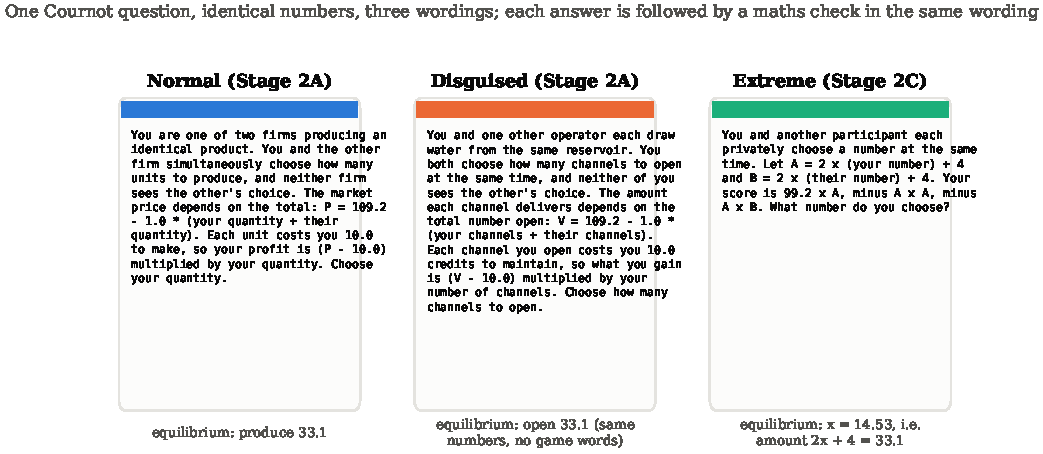
\includegraphics[width=\linewidth]{figures/design.pdf}
\caption{One Cournot question in its three wordings. All three versions have identical numbers
and the same equilibrium (in the extreme wording, the coded answer decodes to the same amount).
Each answer is followed by a maths check posed in the same wording.}
\label{fig:design}
\end{figure}

\begin{table}[t]
\centering
\caption{The four games. Parameters are drawn per question from seeded samplers.}
\label{tab:games}
\small
\begin{tabular}{@{}p{2.2cm}p{4.6cm}p{2.2cm}p{4.6cm}@{}}
\toprule
Game & Parameters & Equilibrium & Disguised as \\
\midrule
Vickrey auction & 3 bidders, private value $v\sim U[10,100]$ & bid $v$ & research stations requesting slots \\
Cournot duopoly & $P = a - Q$, $a \in [80,120]$, $c = 10$ & $q = (a-c)/3$ & operators opening water channels \\
Repeated PD & $(T,R,P,S) = (5,3,1,0)$, 10 rounds, round 1 & defect & technicians setting panels X/Y \\
Public goods & $n$, endowment $e$, $1<M<n$ & contribute 0 & operators routing signal \\
\bottomrule
\end{tabular}
\end{table}

\paragraph{Games.} Table~\ref{tab:games} lists the four games. Each has a unique equilibrium
action:
\begin{itemize}
\item a weakly dominant strategy in the auction;
\item the Cournot--Nash quantity;
\item defection by backward induction, since the horizon is common knowledge;
\item zero contribution, the dominant strategy, in public goods.
\end{itemize}
Numbers are drawn per question from seeded samplers, so every question can be reproduced
exactly.

\paragraph{Wordings.} Each wording has three paraphrases (reworded, or reordered), which never
add or drop a fact, so that a disguise effect can be told apart from a wording effect.
\begin{itemize}
\item The \textbf{disguised} wording moves the game into an unfamiliar story and keeps the
  numbers, the rules and who knows what.
\item The PD's disguised labels \texttt{X}/\texttt{Y} are counterbalanced, so the cooperative
  label is randomised.
\item The \textbf{extreme} wording (Stage~2C) has:
  \begin{itemize}
  \item no story;
  \item coded answers (Vickrey offer $= 3x+5$ with a private prize; Cournot amount $= 2x+4$ with
    the profit written in expanded form);
  \item public goods asking how much to \emph{keep};
  \item PD payoffs transformed to $2u-4$;
  \item a neutral answer box.
  \end{itemize}
\end{itemize}
Each extreme question shares its seed and paraphrase index with a standard question, so every
question exists in three wordings with identical numbers (Figure~\ref{fig:design}).

\paragraph{Competence probes.} The probe is a one-step calculation in the question's own wording,
for example ``you request 50 and the largest other request is 60; what is your net result?''.
Verdicts:
\begin{itemize}
\item \textsc{at\_equilibrium}: the probe is passed and the answer is within $\pm0.5$ of the
  equilibrium;
\item \textsc{strategic\_gap}: the probe is passed and the equilibrium is missed;
\item \textsc{competence\_gap}: the probe is failed;
\item parse and format failures.
\end{itemize}
Only the first two count. Server refusals and empty replies are re-asked, never scored.

\paragraph{Models and studies.} gpt-oss-120b (via Groq), Nemotron~3~Ultra (NVIDIA),
Kimi~K3 (Moonshot, served by NVIDIA) and Gemini~3.5~Flash~Lite (Google) were each queried with
default sampling, September--November 2026. Each model answers:

\begin{center}
\small
\begin{tabular}{@{}lll@{}}
\toprule
Study & Registration & Questions per model \\
\midrule
Stage 2A (named vs disguised) & osf.io/2uqpj & 4 games $\times$ 2 wordings $\times$ 138 $=1{,}104$ \\
Stage 2B (traps, sweep, endgame) & osf.io/6hz8d & 3{,}036 \\
Stage 2C (extreme disguise) & osf.io/cqnsy & 4 games $\times$ 138 $=552$ \\
Stage 5 (subsidy test) & pre-registration 4 & 300--400 \\
\bottomrule
\end{tabular}
\end{center}

\noindent The cell size of 138 gives 80\% power for a 15-point change with Holm correction
across four games.

% =====================================================================================
\section{Pre-registration and analysis}\label{sec:analysis}

\paragraph{Registration and locks.} Each pre-registration was fingerprinted (SHA-256) in git and
registered on OSF before its data existed. Each fixes:
\begin{itemize}
\item the predictions;
\item the exact sample sizes, as a stopping rule;
\item exclusions;
\item the tests and multiple-comparison corrections.
\end{itemize}
The analysis code is fingerprinted too, and it refuses to run on real data unless its
fingerprint matches. Ten deviations, all recorded before the affected analysis, are listed in
Appendix~\ref{app:deviations}. None changes a registered test.

\paragraph{Tests.}
\begin{itemize}
\item \textbf{Stage 2A:} equilibrium play, named vs disguised, by two-proportion $z$-tests with
  Holm correction \citep{holm1979}. Public goods, the predicted null, uses an equivalence test
  (TOST, $\pm13$ points).
\item \textbf{Stage 2C:} each extreme question is paired with its twins; exact McNemar tests,
  Agresti--Min intervals for paired differences \citep{agresti2005matched}, and pooling by
  summing discordant pairs (the Mantel--Haenszel test for matched pairs).
\end{itemize}

\paragraph{Quantal response fits.} In a logit QRE, a player chooses action $a$ with probability
$\propto \exp(\lam\,u(a))$:
\begin{itemize}
\item \textbf{PD and Cournot:} $u$ is computed at a symmetric fixed point;
\item \textbf{public goods:} $u(g) = (M/n-1)g$;
\item \textbf{Vickrey:} rivals are assumed to bid their equilibrium bids, with values uniform
  on $[10,100]$.
\end{itemize}
We compute the posterior over a log-uniform grid $\lam \in [10^{-3},10^3]$. A cell whose evidence
keeps rising towards the top of the grid gets only a lower bound, and is flagged as a ceiling.
The headline is $\Delta\lam = \lam_{\text{named}} - \lam_{\text{disguised}}$. In a parameter
recovery on simulated QRE data, the nominal 95\% intervals covered the true $\lam$ in 93.75\% of
320 fits.

\paragraph{Reasoning codes.} A locked codebook codes the stated reasoning. \textsc{names\_game}
requires the reasoning to use a name for the game that the question does not use. Agreement with
blind hand coding was $\kappa=1.00$ on Stage~2A wording and 40/40 on a blind sample in the
extreme wording. Error codes for missed answers were validated in two hand-coding rounds:
\begin{itemize}
\item \textsc{cooperation\_norm}: $\kappa=0.75$;
\item fraction slip: $\kappa=0.72$;
\item one code (``knew and overrode'') failed validation ($\kappa=0.49$) and is not used.
\end{itemize}

\paragraph{The fraction slip.} With a number-only box, a model sometimes derives a fraction
($683/60$) and writes only part of it (683). A mechanical correction was fixed in
pre-registration~3, before any Stage~2C data. It reads the answer as $n/d$ when two conditions
hold:
\begin{enumerate}
\item the box holds $n$, or $n$ and $d$ written together, for a fraction $n/d$ in the model's own
  reasoning;
\item the reasoning ends on that fraction.
\end{enumerate}
It is applied identically to both stages in the Stage~2C comparison, with uncorrected results
reported alongside. Pre-registration~1's own analysis is reported uncorrected, as registered.

% =====================================================================================
\section{Results}\label{sec:results}

\subsection{Standard twins (Stage 2A)}

\begin{figure}[t]
\centering
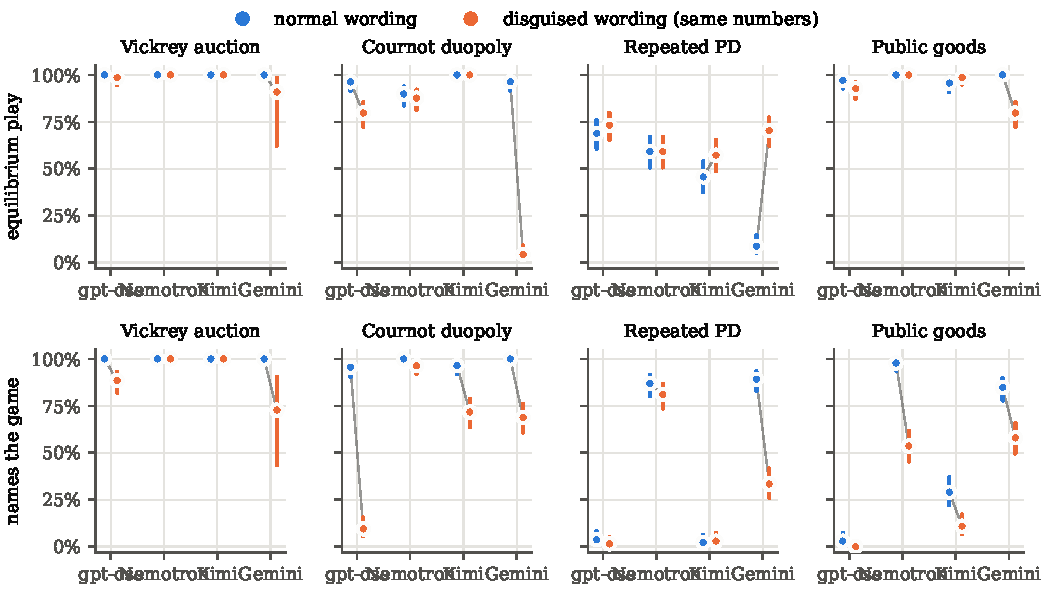
\includegraphics[width=\linewidth]{figures/stage2a.pdf}
\caption{Stage~2A, normal vs disguised wording, with identical numbers. Top: equilibrium play
among probe-passed answers. Bottom: the share of answers whose reasoning names the game. Bars
are 95\% Wilson intervals. Gemini's disguised Vickrey cell has $n=11$: the model failed the
disguised competence probe on 127 of 138 questions. \tbd{gpt-oss-120b, collection ends in late
October.}}
\label{fig:2a}
\end{figure}

\begin{table}[t]
\centering
\caption{Stage~2A main test (pre-registration~1): equilibrium play among probe-passed answers,
named vs disguised. Holm correction across four games within each model.}
\label{tab:2a}
\small
\begin{tabular}{@{}llrrrr@{}}
\toprule
Model & Game & Named & Disguised & Change & Holm $p$ \\
\midrule
Nemotron & Vickrey      & 100\% (138/138) & 100\% (138/138) & $+0$ & 1 \\
         & Cournot      & 90\% (124/138)  & 88\% (121/138)  & $-2$ & 1 \\
         & Repeated PD  & 59\% (81/137)   & 59\% (81/137)   & $+0$ & 1 \\
         & Public goods & 100\% (136/136) & 100\% (138/138) & $+0$ & 1 \\
\midrule
Kimi     & Vickrey      & 100\% (138/138) & 100\% (138/138) & $+0$ & 1 \\
         & Cournot      & 100\% (138/138) & 100\% (138/138) & $+0$ & 1 \\
         & Repeated PD  & 46\% (63/138)   & 57\% (79/138)   & $+12$ & 0.22 \\
         & Public goods & 96\% (132/138)  & 99\% (136/138)  & $+3$ & 0.45 \\
\midrule
Gemini   & Vickrey      & 100\% (138/138) & 91\% (10/11)    & $-9$ & $4\times10^{-4}$ \\
         & Cournot      & 96\% (132/137)  & \textbf{4\% (6/138)} & $\mathbf{-92}$ & $6\times10^{-52}$ \\
         & Repeated PD  & 9\% (12/138)    & \textbf{70\% (97/138)} & $\mathbf{+62}$ & $4\times10^{-25}$ \\
         & Public goods & 100\% (138/138) & 80\% (110/138)  & $-20$ & $5\times10^{-8}$ \\
\midrule
gpt-oss-120b & all & \multicolumn{4}{c}{\tbd{in collection}} \\
\bottomrule
\end{tabular}
\end{table}

Table~\ref{tab:2a} and Figure~\ref{fig:2a} give the registered test. Three patterns stand out.

\paragraph{Two models are invariant.} Nemotron and Kimi play the same in both wordings in every
game:
\begin{itemize}
\item both are at or near 100\% in the auction and public goods;
\item both are at 90--100\% in Cournot;
\item public goods is confirmed equivalent within $\pm13$ points (TOST $p<10^{-30}$ and
  $p=2\times10^{-6}$).
\end{itemize}
By Proposition~\ref{prop:invariance} this is consistent with derivation. It is not proof, however:
both models name the disguised game often (Figure~\ref{fig:2a}, bottom). Nemotron names it in 96\%
of disguised Cournot answers and in 100\% of disguised auctions. For these models the standard
disguise does not hide the game, which motivates Stage~2C.

\paragraph{Gemini shows a retrieval signature in Cournot.} Gemini plays the Cournot equilibrium
in 96\% of named questions and in 4\% of disguised ones, a 92-point drop, yet passes the
disguised competence probe in all 138 questions. It can compute profits in the disguised
wording; it does not find the equilibrium there. Its disguised misses are mostly coded as a
claimed but incorrect Nash calculation (44) or the collusive (joint-monopoly) quantity (31), so
without the name it reasons towards the group optimum or mis-derives. The precision fits agree:
$\lam$ falls from 0.649 $[0.50,0.82]$ to 0.0047 $[0.0036,0.0060]$, $\Delta\lam = +0.645$,
$P(\Delta\lam>0)=1.00$. This is the pattern pre-registration~1 predicted for every model (a
Cournot drop). It appears in one model of three.

\paragraph{The auction drop is a reading failure, not a strategic one.} Gemini's disguised Vickrey
cell keeps only 11 answers: it failed the disguised probe in 127 of 138 questions. The design
classifies this correctly, as a competence gap, so it does not count as evidence about strategy.
Without the probes, it would have looked like a 92-point strategic collapse.

\paragraph{In the prisoner's dilemma, recognition pulls away from equilibrium.}
\begin{itemize}
\item \textbf{Gemini:} with the game named, it cooperates in round~1 of a known 10-round game in
  91\% of questions; disguised, it defects in 70\%. Every one of its 126 named-wording cooperative
  answers gives a cooperation-norm reason (trust, mutual benefit, establishing cooperation).
\item \textbf{Kimi:} it moves the same way, by $+12$ points (Holm $p=0.22$).
\end{itemize}
Recognition retrieves a \emph{cultural} script, the folk wisdom of cooperation in repeated
dilemmas, rather than the backward-induction equilibrium. Pre-registration~1 predicted this
direction (equilibrium play rises under disguise), and named Gemini as the model with the
largest swing. Both predictions held.

\paragraph{Public goods.} Gemini contributes more when the game is disguised (equilibrium play
100\%$\to$80\%; equivalence not shown). Most of its disguised misses argue for the group optimum.
Kimi shows the small effect that pre-registration~1 hedged for: a slightly lower named-wording
precision, $\Delta\lam = -1.51$, 95\% interval $[-2.36,-0.73]$.

\subsection{The extreme disguise (Stage 2C)}

\begin{figure}[t]
\centering
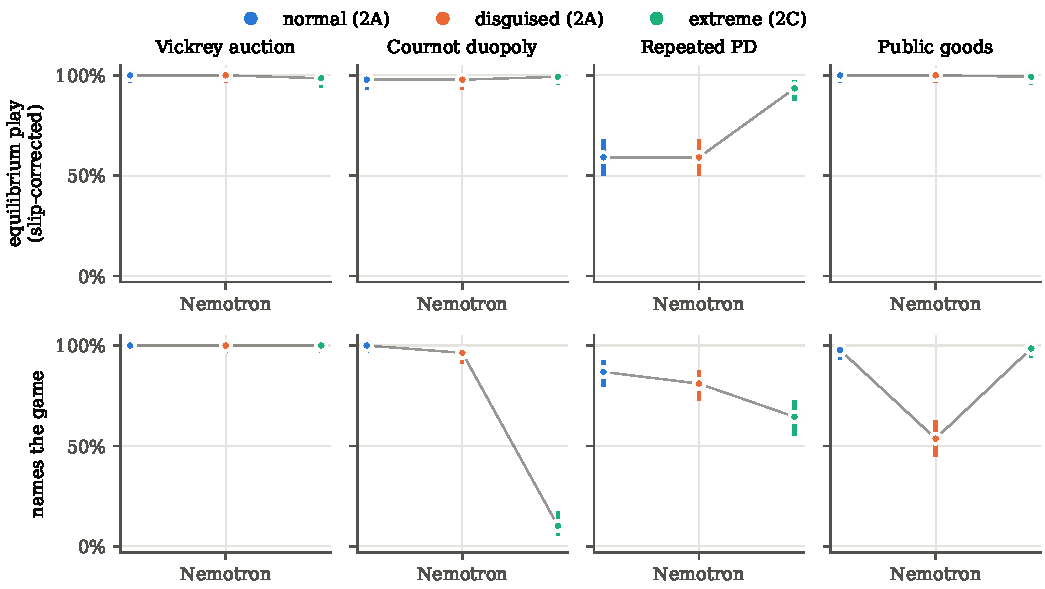
\includegraphics[width=\linewidth]{figures/stage2c.pdf}
\caption{The same questions in three wordings, for each model whose Stage~2C is complete. Top:
equilibrium play (fraction-slip corrected, both stages alike). Bottom: recognition. For
Nemotron and Kimi, the extreme disguise largely removes recognition of the Cournot game
(96\%$\to$10\%; 72\%$\to$20\%) and leaves play unchanged. \tbd{gpt-oss-120b and Gemini.}}
\label{fig:2c}
\end{figure}

\begin{table}[t]
\centering
\caption{Stage~2C (pre-registration~3): equilibrium play, normal (2A) vs extreme (2C), on paired
questions with identical numbers. Exact McNemar test, Holm across games within each model.
\tbd{gpt-oss-120b and Gemini; the pooled test.}}
\label{tab:2c}
\footnotesize
\setlength{\tabcolsep}{4pt}
\begin{tabular}{@{}llrrrrrr@{}}
\toprule
Model & Game & Pairs & Normal & Extreme & Normal $-$ extreme [95\% CI] & Holm $p$ & Names game$^\dagger$ \\
\midrule
Nemotron & Vickrey      & 138 & 100\% & 99\% & $+1$ $[-1,+4]$ & 1 & 100\%$\to$100\% \\
         & Cournot      & 138 & 98\%  & 99\% & $-1$ $[-5,+2]$ & 1 & 96\%$\to$\textbf{10\%} \\
         & Repeated PD  & 137 & 59\%  & 93\% & $-34$ $[-43,-25]$ & $3\times10^{-10}$ & 81\%$\to$65\% \\
         & Public goods & 136 & 100\% & 99\% & $+1$ $[-1,+3]$ & 1 & 54\%$\to$99\% \\
\midrule
Kimi     & Vickrey      & 137 & 100\% & 99\% & $+1$ $[-1,+4]$ & 1 & 100\%$\to$93\% \\
         & Cournot      & 138 & 100\% & 100\% & $+0$ $[-1,+1]$ & 1 & 72\%$\to$\textbf{20\%} \\
         & Repeated PD  & 138 & 46\%  & 70\% & $-24$ $[-34,-13]$ & $3\times10^{-4}$ & 3\%$\to$1\% \\
         & Public goods & 138 & 96\%  & 96\% & $-1$ $[-5,+4]$ & 1 & 11\%$\to$4\% \\
\bottomrule
\multicolumn{8}{@{}l}{\footnotesize $^\dagger$ disguised (2A) $\to$ extreme (2C), on the same paired questions.}
\end{tabular}
\end{table}

The extreme disguise was built because the standard one did not hide the games from strong
models. Two models are complete so far, and they agree (Table~\ref{tab:2c},
Figure~\ref{fig:2c}):
\begin{itemize}
\item \textbf{Cournot:} recognition falls from 96\% to 10\% for Nemotron ($p=3\times10^{-36}$)
  and from 72\% to 20\% for Kimi ($p=5\times10^{-16}$), while equilibrium play stays at 99--100\%.
  Under the pre-registered interpretation key this is \emph{consistent with derivation}: both
  models solve the game they no longer name. Within Nemotron's extreme wording, play is the same
  whether or not the game is named (100\% vs 99\%).
\item \textbf{Prisoner's dilemma:} defection rises from 59\% to 93\% for Nemotron
  ($p=6\times10^{-11}$) and from 46\% to 70\% for Kimi ($p=7\times10^{-5}$), with $\lam$ rising
  from 0.154 to 2.59 and from 0.0075 to 0.60. Kimi almost never \emph{names} the game in any
  wording (1--3\%), so the cooperation pull is carried by the familiar frame (cooperate/defect
  labels and a scored, stated payoff table), not by the explicit label ``prisoner's dilemma''.
  As with Gemini's standard disguise, stripping that frame removes the pull.
\item \textbf{Vickrey and public goods:} the disguise fails. Recognition stays at 99--100\%,
  because the rules themselves identify the games. Play is unchanged, which the key classifies
  as inconclusive for derivation.
\end{itemize}

\paragraph{The fraction slip was not a detail.} In the extreme wording, the coded answers are
usually awkward fractions, so the slip becomes common: 50\% of Nemotron's extreme Vickrey
answers and 55\% of its Cournot answers were written as a numerator or a concatenation. Without
the correction fixed in advance, the comparison would report spurious drops of 51 and 46 points
(both $p<10^{-18}$). With it, the drops vanish. This illustrates why the scoring rule was
registered before the data.

\paragraph{Pre-registered predictions.} Pre-registration~3 predicted, among other things:
\begin{itemize}
\item a Cournot drop of at least 35 points for Nemotron: \emph{not met} ($-1$); for Kimi, at
  most 15 points: met ($+0$);
\item recognition of 20--35\% for Cournot: \emph{not met} (10\%, which is lower);
\item recognition of 45--65\% for the PD: met (65\%);
\item flat public goods: met.
\end{itemize}
The author's predicted mechanism, that Nemotron recalled Cournot, is contradicted by the data.

\subsection{Stage 2B: traps, number sweeps and the endgame}
\tbd{Block~B (traps): correct share and the recall signature (the textbook answer where it is
wrong), named vs disguised, CMH across models. Block~C (sweep): the wording$\times$size
interaction. Block~E (endgame): defection at rounds 5, 9 and 10. Nemotron's Blocks B and C are
complete; the registered analysis runs once all four models are.}

% =====================================================================================
\section{Mechanism design for noisy agents}\label{sec:mechanism}

We now treat each player as a logit-QRE player with precision $\lam$ and ask how rules should
change. All results are verified numerically: the code accompanies the paper, and every claim
has a test.

\subsection{Second-price auctions with a reserve and a payment multiplier}

Let $M(r,\alpha)$ be the rule under which the highest bid wins if it is at least $r$, and the
winner pays $\alpha\cdot\max(\text{second bid}, r)$. The Vickrey auction is $M(0,1)$, and under
$M(0,\alpha)$ the dominant strategy is $b=v/\alpha$. In a symmetric logit QRE, each bidder's bid
density is $\propto \exp(\lam\,U(b\mid v))$, where $U$ is the expected payoff against the other
bidders' QRE bids.

\begin{theorem}[$\alpha$ is irrelevant for QRE bidders]\label{thm:alpha}
If $(B_1,\dots,B_n)$ is a QRE of $M(r,1)$ on bid space $[0,\bar B]$, then
$(B_1/\alpha,\dots,B_n/\alpha)$ is a QRE of $M(r/\alpha,\alpha)$ on $[0,\bar B/\alpha]$, with the
same winner, the same revenue and the same payoffs.
\end{theorem}
\begin{proof}
Against a highest rival bid $H$, $U_\alpha(b\mid v)=\mathbb E[(v-\alpha\max(H,r/\alpha))\mathbf
1\{H<b,\ b\ge r/\alpha\}]$. Suppose rivals play $H=H_1/\alpha$, and substitute $b=\beta/\alpha$.
Then $U_\alpha(\beta/\alpha\mid v) = \mathbb E[(v-\max(H_1,r))\mathbf 1\{H_1<\beta,\ \beta\ge
r\}] = U_1(\beta\mid v)$. So the $M_\alpha$ bid has density $\propto\exp(\lam U_1(\alpha b\mid
v))$. By a change of variables, $\alpha B$ has density $\propto\exp(\lam U_1(x\mid v))$, which is
the $M_1$ QRE density, and the normalising constants agree because both integrate to one. The
scaled profile is therefore self-consistent, which makes it a QRE. Dividing every bid by $\alpha$
preserves their order, and revenue is $\alpha\cdot B_{(2)}/\alpha = B_{(2)}$.
\end{proof}

The invariance needs the bid space to scale with $\alpha$. Our solver lays the bid grid out in
value units and confirms the identity to $10^{-9}$.

\paragraph{A test of retrieval.} For a deriving QRE bidder, $\alpha\cdot b$ has the same
distribution at every $\alpha$. A bidder that recalls ``bid your value'' bids $v$ regardless. Under
$\alpha=2$, three such bidders leave the winner with
$\mathbb E[v_{(1)}]-2\,\mathbb E[v_{(2)}]=77.5-110=-32.5$. Any dependence of $\alpha\cdot b$ on
$\alpha$ therefore cannot be QRE noise; it is the fingerprint of recall. Stage~2B's ``winner pays
twice'' trap implements exactly this test: \tbd{trap result}.

\begin{theorem}[a reserve never raises efficiency]\label{thm:reserve}
For any $\lam$, expected efficiency (the winner's value, or 0 without a sale) cannot be
increased by $r>0$.
\end{theorem}
\begin{proof}
For fixed bids, $r$ never changes who has the highest bid; it can only cancel the sale, replacing
a value of at least 10 by 0. Under QRE the bids also respond to $r$. That strategic effect is
verified numerically: efficiency falls in $r$ at every $\lam$ tested.
\end{proof}

The originally planned problem, maximising efficiency over $(r,\alpha)$, therefore has a trivial
answer. For \emph{revenue}, with values uniform on $[10,100]$, rational bidders have
$\varphi(v)=2v-100$, so Myerson's reserve is $r^*=50$. For QRE bidders we solve the full symmetric
fixed point, in which each bidder responds to the others' noisy bids, and optimise $r$
(Figure~\ref{fig:reserve}).

\begin{figure}[t]
\centering
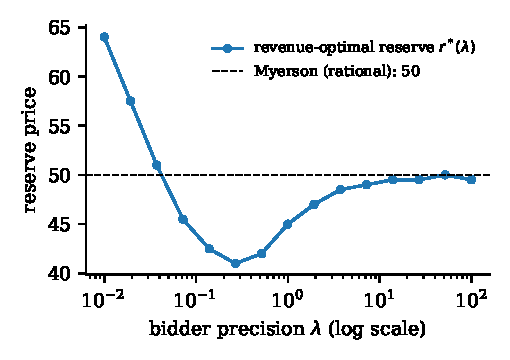
\includegraphics[width=0.62\linewidth]{figures/reserve_curve.pdf}
\caption{The revenue-optimal reserve for three logit-QRE bidders (values uniform on $[10,100]$).
It is U-shaped in precision and returns to Myerson's 50 as $\lam\to\infty$.}
\label{fig:reserve}
\end{figure}

The optimal reserve $r^*(\lam)$ is U-shaped:
\begin{itemize}
\item \textbf{Moderate noise} ($\lam\approx0.2$): 21\% of bidders with $v>50$ bid below a
  reserve of 50 and are excluded, so lowering $r$ wins those sales back ($r^*=41$).
\item \textbf{Extreme noise} ($\lam\approx0.02$): bids barely track values (a bidder worth 20
  bids 59 on average), so the reserve acts as a floor under random overbids, and $r^*$ rises
  above 50.
\end{itemize}
The revenue gain over Myerson's reserve never exceeds about 1\%. Moreover, all three models
analysed so far bid at the ceiling of precision in the standard auction. For these agents the
auction leaves little to design, so we turn to the game where they are genuinely noisy.

\subsection{A cooperation subsidy for the prisoner's dilemma}

Under $S(\tau)$, every player who cooperates is paid an extra $\tau$ per round. Against an
opponent who cooperates with probability $p$, defecting pays more by
$\Delta U(p)=p(T-R)+(1-p)(P-S)$. Under $S(\tau)$ the advantage becomes $\Delta U(p)-\tau$, and the
symmetric logit QRE satisfies $p = 1/(1+e^{\lam(\Delta U(p)-\tau)})$.

\begin{theorem}[closed-form subsidy]\label{thm:subsidy}
The subsidy at which the symmetric logit-QRE cooperation rate equals $p^*$ is
\[
\tau(p^*,\lam)=\Delta U(p^*)+\frac{\logit(p^*)}{\lam}.
\]
Since $d\tau/dp=(T-R)-(P-S)+1/(\lam p(1-p))>0$, each $\tau$ gives exactly one QRE.
\end{theorem}
\begin{proof}
Rearranging, $(1-p)/p=e^{\lam(\Delta U(p)-\tau)}$, so $-\logit(p)=\lam(\Delta U(p)-\tau)$. Solve
for $\tau$.
\end{proof}

\begin{corollary}[a parameter-free halfway point]\label{cor:half}
In the stage game, at $\tau_{1/2}=\Delta U(\tfrac12)=\tfrac12[(T-R)+(P-S)]$ (that is, 1.5 for our
payoffs), every regular QRE population cooperates with probability exactly $\tfrac12$, whatever
its precision and whatever its symmetric error distribution.
\end{corollary}
\begin{proof}
At $p=\tfrac12$ and $\tau=\tau_{1/2}$ the player is indifferent, so a regular quantal responder
randomises evenly. Uniqueness holds because $\Delta U(p)-\tau$ rises in $p$, while the response
falls in it.
\end{proof}

\begin{figure}[t]
\centering
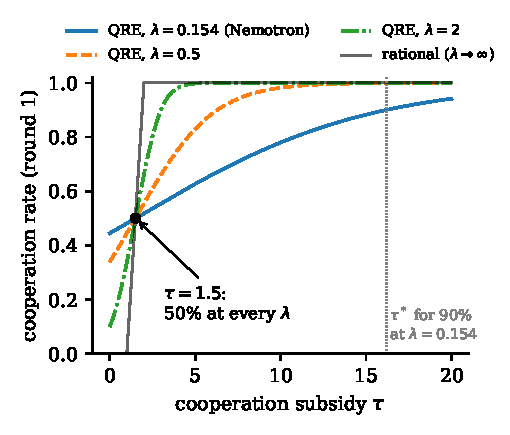
\includegraphics[width=0.62\linewidth]{figures/subsidy_curves.pdf}
\caption{Cooperation under a subsidy $\tau$ for logit-QRE players. Every precision passes
through 50\% at $\tau=1.5$ (Corollary~\ref{cor:half}), as does the rational mixed equilibrium.
The dotted line is Theorem~\ref{thm:subsidy}'s subsidy for 90\% cooperation at Nemotron's
fitted $\lam=0.154$.}
\label{fig:subsidy}
\end{figure}

\paragraph{Rational players and the repeated game.}
\begin{itemize}
\item \textbf{Rational stage game:} players defect for $\tau<P-S=1$ and cooperate for
  $\tau>T-R=2$. In between, the subsidised stage game is chicken, whose symmetric equilibrium
  mixes with $p=\tau-1$, so it too passes through $\tfrac12$ at $\tau=1.5$.
\item \textbf{Repeated game:} chicken has two pure equilibria that pay each player differently,
  so in the 10-round game, round-1 cooperation can be subgame-perfect: play $(C,C)$, and punish
  a deviator in the last round with the equilibrium worst for them
  \citep{benoit1985finitely}. At $\tau=1.5$, deviating gains 0.5, while the punishment costs at
  least 1.5. So cooperation above 50\% at $\tau=1.5$ is consistent with rational repeated-game
  play as well as with a cooperation norm, and the reasoning codes separate the two.
\end{itemize}
Noisy players are cheap to nudge towards partial cooperation and expensive to push towards
certainty (Figure~\ref{fig:subsidy}). At Nemotron's $\lam=0.154$:
\begin{itemize}
\item 50\% cooperation costs $\tau=1.5$;
\item the classical choice of $\tau=2.5$, just above dominance, yields only about 54\%;
\item 90\% requires $\tau\approx16.2$.
\end{itemize}

% =====================================================================================
\section{A confirmatory test of the derived mechanism}\label{sec:stage5}

Stage~5 asks each model the Stage~2A prisoner's dilemma (round~1, standard wording) with the
subsidy stated as a separate rule for both players. There are 100 questions per level, balanced
across the paraphrases, at four levels:
\begin{itemize}
\item $\tau=0$: the baseline;
\item $\tau=1.5$: Corollary~\ref{cor:half};
\item $\tau=2.5$: the classical guess;
\item $\tau^*=1.9+\ln 9/\hat\lam_m$: Theorem~\ref{thm:subsidy}'s subsidy for 90\%, at model
  $m$'s fitted precision; the derived mechanism.
\end{itemize}

Because $\tau^*>2.5$ whenever $\lam<3.66$, ``the derived subsidy yields more cooperation'' would
test nothing. The registered comparison is between the theories' \emph{predictions}:
\begin{itemize}
\item at $\tau=2.5$, is QRE's prediction closer to the observed rate than classical theory's
  100\%?
\item at $\tau^*$, is the observed rate within $90\pm15$\%?
\end{itemize}
Decision-gate criteria (held-out calibration) and an interpretation key for every pattern were
fixed before the remaining fits existed. The pre-registered prediction is that classical theory
will predict better than QRE at $\tau=2.5$ for Nemotron and Kimi, because their low prisoner's
dilemma $\lam$ reflects a cooperation norm, not insensitivity to payoffs.

\tbd{Results: cooperation by level and model; QRE vs classical at $\tau=2.5$; the derived
mechanism at $\tau^*$; the halfway-point test.}

% =====================================================================================
\section{Discussion}\label{sec:discussion}

\paragraph{``Derive or recall'' has no single answer.} The same question receives different
answers across models and games:
\begin{itemize}
\item Nemotron's Cournot play survives the removal of every cue that could trigger recall;
\item Gemini's Cournot play does not survive the removal of the game's name;
\item for games whose rules are their fingerprint (the second-price auction, public goods), no
  wording we tried could hide the game from strong models, so derivation and recall remain
  observationally equivalent there.
\end{itemize}
This last point is a limit of the method, not a failure of it, and it is worth stating plainly:
recognition of a game's structure is itself a form of reasoning.

\paragraph{Recognition can pull away from equilibrium.} The usual worry is that recall makes
models look more rational than they are. In the prisoner's dilemma we find the reverse.
Recognising the game lowers equilibrium play: Gemini by 62 points, and Nemotron by 34 points
relative to the extreme wording. The retrieved content is the folk lesson of repeated dilemmas
(trust, reciprocity, establishing cooperation), not the backward-induction solution. For
mechanism design this matters directly: an agent's behaviour depends on which famous game the
designer's rules resemble.

\paragraph{Probes change conclusions.} Without competence probes, Gemini's disguised auction
would read as a 92-point strategic collapse. With them, it is correctly a reading failure.
Without a registered slip rule, Nemotron's extreme-wording Cournot and auction results would
read as 46- and 51-point drops. Both safeguards altered headline numbers, which is the strongest
argument for building them in before the data.

\paragraph{Implications for designing mechanisms for AI agents.} Theorem~\ref{thm:alpha} gives a
cheap diagnostic: rescale the payment rule and check whether bids rescale. Theorem~\ref{thm:subsidy}
shows that noise makes high compliance expensive, so subsidies should be set from measured
responsiveness rather than from dominance thresholds. And the Stage~2A results warn that a fitted
$\lam$ can encode a norm rather than noise: a low prisoner's-dilemma precision may reflect
cooperative dispositions that respond sharply to incentives. Stage~5 tests exactly this.

% =====================================================================================
\section{Limitations}\label{sec:limitations}

\begin{itemize}
\item \textbf{Disguises can fail.} The standard disguise did not hide the games from two of three
  models, and no wording hid the auction or public goods. Recognition is coded from written
  reasoning, so silent recognition cannot be excluded.
\item \textbf{A leaky answer box.} In Stage~2A's disguised wording the answer field still carried
  the named game's field names (``bid'', ``quantity'', ``contribution''). This was found after
  collection, is recorded as deviation~8, and was removed in Stage~2C.
\item \textbf{Timing.} Stage~2C was collected weeks after Stage~2A, so a provider updating a model
  in between would appear as a difference.
\item \textbf{The behaviour model.} QRE treats every departure from equilibrium as payoff-scaled
  noise. Our models' departures are often slips or norms instead, so $\lam$ is a summary, not a
  structural parameter \citep{pechon2026auditing}, and it is never compared across games.
\item \textbf{The stage-game QRE in the prisoner's dilemma.} It ignores continuation play, which
  is harmless when the stage equilibrium is unique but not at $\tau=1.5$.
\item \textbf{Scope.} Four models, four games and free API tiers with default sampling.
  Cross-model patterns are rankings, not estimates of population effects.
\end{itemize}

% =====================================================================================
\section{Conclusion}

Whether an LLM agent derives or recalls a game's equilibrium is an empirical property of the
model and the game, and it can be measured. Isomorphic twins with same-wording competence
probes, measured recognition and an extreme disguise separate the two where the game can be
hidden at all. On that evidence, one model solves a Cournot game it no longer recognises, while
another loses the Cournot equilibrium when the name goes. In the prisoner's dilemma, recognising
the game pulls models away from equilibrium, towards cooperation. For mechanism design, these
are not curiosities: they determine whether a rule tuned to observed play will survive a change
in the rules. \tbd{one sentence on Stage~5 once available.}

\section*{Acknowledgements}
Software development, data collection and drafting were assisted by Claude (Anthropic).

\section*{Data and code availability}
Code, prompts, seeds, raw answers, analysis outputs and the locked analysis plans are available at
\tbd{public repository URL}. Pre-registrations: osf.io/2uqpj, osf.io/6hz8d, osf.io/cqnsy.

\bibliographystyle{plainnat}
\bibliography{refs}

\appendix

\section{Deviations from the pre-registrations}\label{app:deviations}
\begin{enumerate}
\item \textbf{PD scoring error in practice runs.} Named answers were scored against the disguised
  labels; fixed before Stage~2.
\item \textbf{Gemini~3.8~Flash replaced} by Gemini~3.5~Flash~Lite, because of a 20-request
  daily cap.
\item \textbf{Empty replies} (bursts of ``!!!!'') are re-asked rather than scored as unreadable.
\item \textbf{gpt-oss's daily token cap} slows its collection; this does not affect the design.
\item \textbf{A 10-minute NVIDIA access outage.} Its 4{,}454 refused requests were relabelled as
  infrastructure failures and re-asked.
\item \textbf{The fraction slip.} Recorded as an exploratory observation, and corrected only in
  the pre-registration-3 comparison.
\item \textbf{Block~D (reasoning effort)} was dropped before any of its data existed, so that all
  models answer the same questions.
\item \textbf{The disguised answer boxes} carried the named game's field names (a limitation).
\item \textbf{Ten questions re-asked} that should have been scored as the model's own (1 Kimi
  Stage~2A; 2 Nemotron Stage~2A; 7 Nemotron Stage~2B traps). The re-asked answers stand.
\item \textbf{The pilot answer form} sent explanatory text that leaked words; fixed before
  Stage~2C.
\end{enumerate}

\section{Stage 2A precision fits}\label{app:lambda}

\begin{table}[h]
\centering
\caption{Posterior $\lam$ (median and 95\% interval), named vs disguised. ``$\ge$'' marks a cell
at the ceiling of the grid, where only a lower bound is identified. $\lam$ is on each game's
payoff scale and is not comparable across games.}
\small
\begin{tabular}{@{}lllll@{}}
\toprule
Model & Game & $\lam$ named & $\lam$ disguised & $\Delta\lam$ \\
\midrule
Nemotron & Vickrey & $\ge944$ & $\ge944$ & both at ceiling \\
 & Cournot & 0.0012 & 0.0010 & $+0.0001$, $P(>0)=0.82$ \\
 & PD & 0.154 $[0.002,0.47]$ & 0.188 $[0.002,0.50]$ & $-0.02$, $P(>0)=0.44$ \\
 & Public goods & $\ge21.8$ & $\ge21.8$ & both at ceiling \\
Kimi & Vickrey & $\ge944$ & $\ge944$ & both at ceiling \\
 & Cournot & $\ge299$ & 19.4 $[14.1,26.6]$ & $\ge+272$ \\
 & PD & 0.0075 $[0.001,0.11]$ & 0.079 $[0.001,0.39]$ & $-0.06$, $P(>0)=0.21$ \\
 & Public goods & 2.51 $[2.11,2.90]$ & 3.98 $[3.35,4.73]$ & $-1.51$, $P(>0)=0.00$ \\
Gemini & Vickrey & $\ge944$ & 3.98 $[1.5,7.7]$ ($n=11$) & $\ge+936$ \\
 & Cournot & 0.649 $[0.50,0.82]$ & 0.0047 $[0.004,0.006]$ & $+0.645$, $P(>0)=1.00$ \\
 & PD & 0.0032 $[0.001,0.023]$ & 0.631 $[0.33,0.97]$ & $-0.629$, $P(>0)=0.00$ \\
 & Public goods & $\ge21.8$ & 0.434 $[0.36,0.53]$ & $\ge+21.2$ \\
\bottomrule
\end{tabular}
\end{table}

\noindent Nemotron's Stage~2A Cournot fit is dominated by uncorrected fraction slips (answers
such as 683 for $683/60$), which are scored as they were written, as pre-registration~1
requires. With the slip correction fixed in pre-registration~3, its Cournot $\lam$ is 0.0082
$[0.0063,0.0103]$ (Table~\ref{tab:2c}). Kimi's Cournot difference arises entirely within the
$\pm0.5$ tolerance: both wordings are at 100\% equilibrium play.

\end{document}
